\documentclass{article}
\usepackage[utf8]{inputenc}
\usepackage{graphicx}
\usepackage{tikz}
\usepackage{lipsum} % Paquete para generar texto de relleno
\usepackage{fancyhdr} % Paquete para encabezados y pies de página
\usepackage[left=3cm, right=3cm, top=2.5cm, bottom=2.5cm]{geometry} % Paquete para ajustar los márgenes
\usepackage{tocloft} % Para personalizar el índice
\usepackage{parskip} % Para añadir espacios entre párrafos
\usepackage{minted}
\usepackage{xcolor} % Paquete para usar colores
\usepackage{grffile}
\usepackage{natbib} % Paquete para estilo de citas
\usepackage{tabularx}
\usepackage{changepage}
\usepackage{amsmath}
\usepackage{tikz}
\usepackage{adjustbox}

\usetikzlibrary{automata, positioning}

%Definitions
\definecolor{lightgray}{gray}{0.5}

\renewcommand{\contentsname}{Índice}
\renewcommand{\cfttoctitlefont}{\hfill\Large\bfseries}
\renewcommand{\cftsecleader}{\cftdotfill{\cftdotsep}} % Rellena con puntos las secciones
\renewcommand{\cftsubsecleader}{\cftdotfill{\cftdotsep}} % Rellena con puntos las subsecciones
\renewcommand{\cftaftertoctitle}{\par\noindent\hrulefill\par\nobreak\vskip -0.5\baselineskip}

\newcommand{\horasVhdl}[2]{\textbf{Horas invertidas en el diseño de VHDL:} Iván D.: #1, Víctor M.P: #2\par\nointerlineskip}
\newcommand{\horasEntenderEnunciado}[2]{\textbf{Horas invertidas en entender el enunciado proporcionado:} Iván D.: #1, Víctor M.P: #2\par\nointerlineskip}
\newcommand{\horasDepuracion}[2]{\textbf{Horas invertidas en depurar el proyecto en busca de fallos:} Iván D.: #1, Víctor M.P: #2\par\nointerlineskip}
\newcommand{\horasMemoria}[2]{\textbf{Horas invertidas en el desarrollo de la memoria del proyecto:} Iván D.: #1, Víctor M.P: #2\par\nointerlineskip}

\fancypagestyle{plain}{
    \fancyhf{}
    \renewcommand{\headrulewidth}{0pt} % Elimina la línea de encabezado
    \fancyfoot[R]{\thepage} % Número de página a la derecha
}

% Configuración del encabezado y pie de página
\pagestyle{fancy}
\fancyhf{} % Limpia los encabezados y pies de página predeterminados
\renewcommand{\footrulewidth}{0.4pt}
\fancyfoot[L]{\textit{AOC - Proyecto 2}} % Encabezado izquierdo con el título del proyecto
\fancyhead[L]{\textit{Iván Deza, Víctor Martinez}}
\fancyfoot[R]{\thepage} % Pie de página centrado con el número de página
\renewcommand{\footrule}{\hbox to\headwidth{\color{lightgray}\leaders\hrule height \headrulewidth\hfill}}
\renewcommand{\headrule}{\hbox to\headwidth{\color{lightgray}\leaders\hrule height \headrulewidth\hfill}}


\begin{document}

\begin{titlepage}
    \centering
    \vspace*{\fill}
    \begin{figure}[htbp]
        \centering
        \begin{tikzpicture}[remember picture ,overlay]
          \node[opacity=0.1,inner sep=0pt, rotate=30] at (0, -6) {
\includegraphics[width=0.90\paperwidth]{assets/unizar.png}}; % Cambia "tu_logo.png" por el nombre de tu archivo de imagen del logo
        \end{tikzpicture}
    \end{figure}
    \vspace*{\fill}
    
    {\scshape\LARGE Universidad de Zaragoza \par}
    \vspace{0.5cm}
    \rule{\linewidth}{0.5mm} % Línea horizontal
    \vspace{0.5cm}
    {\scshape\Large Departamento de Organización de Computadoras \par}
    \vspace{0.5cm}
    \rule{\linewidth}{0.5mm} % Línea horizontal
    \vspace{1.5cm}
    {\huge\bfseries AOC - Proyecto 2\par}
    \vspace{0.5cm}
    {\Large\itshape Jerarquía de Memoria \par}
    \vspace{2cm}
    {\Large\itshape Iván Deza y Víctor Martinez \par}
    \vspace{0.5cm}
    {\Large\itshape José L. Briz, Javier Resano y Alejandro Valero \par}
    \vfill
    % Agrega la fecha si lo deseas
    {\large \today\par}
\end{titlepage}

\newpage

\tableofcontents

\newpage
\section{Introducción}
El proyecto en cuestión trata de el diseño e implementación de una unidad de control que sea capaz de controlar una jerarquía de memoria
donde tenemos: una memoria cache, de rápido acceso, una memoria Scratch de datos, también de acceso rápido, además de una memoria principal más lenta que las anteriores mencionadas.
Esta jerarquía de memoria viene conectada vía un bus, de tipo semisincrono, que actúa de árbitro entre todas las memorias de la jerarquía. Además la política de funcionamiento de la cache es \textbf{Fetch on Write Miss} (traemos el bloque que necesitamos cuando hay un fallo de escritura)
y \textbf{Copy Back} (no actualizamos escrituras a la memoria principal instantáneamente si no cuando hay un fallo y nos deshacemos de ese bloque). Además de todo esto, la política de reemplazo es de tipo FIFO (First In First Out). \par
Esta jerarquía de memoria se introduce en el chip MIPS del proyecto número 1, al cual se le ha cambiado el MD subsystem por uno más complejo, el cual incluye una jerarquía de memoria.\par
Además de esto, en el apartado 8.1, hemos comentado como funciona un ataque de canal lateral a una memoria cache, demostrado su funcionamiento y creado una prueba de concepto para este tipo de ataques. También se propone una estrategia para mitigar esta vulnerabilidad.

\section{Diagrama de Estados de la UC}
Aquí se adjunta una imagen con el diagrama de estados de la unidad de control que hemos implementado. Este diseño tiene política de escritura \textbf{Copy Back} la cual consiste
en que no se escribe en memoria principal todos los cambios que se han ido haciendo durante el programa, si no que se actualiza solo en el momento en el que se bloque se expulsa
de la memoria cache. Este hace que la carga de trabajo de entrada salida sea menor ya que reducimos en gran medid los accesos de escritura a memoria principal. Además, ya que la 
memoria cache es más rápida que la memoria principal, hace que se reduzca el tiempo de ejecución de ciertas secuencias de instrucciones como bucles.\par
Otra politica utilizada es la denominada \textbf{Fetch on Write Miss}, la cual consiste en que traemos a cache los datos en caso de que halla un fallo de escritura. Esto complementa
muy bien la política copy back y hace que el rendimiento de la cache sea superior a otro conjuntos de politicas como Write Through junto a una política que implemente Fetch on Write miss.\cite{RivoireCacheWrite}\par
\par 
En resumen,esta unidad de control cuenta con 4 estados diferentes, el primero de ellos es inicio, donde gestionamos, tanto los hits como los errores de alineamiento. En el segundo estado
, al cual hemos llamado bus request, lo que hacemos es pedir el bus, si devsel es 0, significa que la direccion no es de ninguna de las memorias conectadas y volveremos a inicio actualizando el error. 
En caso de que algun servidor actualice devsel y lo recibamos a 1, pasamos al estado de transferencia, en el cual mandaremos la dirección a través del bus. 
A partir de aquí ya diferenciaremos entre fallo limpio, fallo sucio, o que sea para la memoria Scratch. En caso de que sea un miss sucio, mandaremos la dirección en la cual querremos escribir el el bloque sucio de MC en memoria principal
para acutalizar esta. Una vez se ha hecho la transferencia del bloque sucio, estaremos en un caso de fallo limpio entonces podemos ir al estado de fallo limpio donde se gestiona traer de memoria el bloque necesario.


\begin{center}
\begin{adjustbox}{left} 
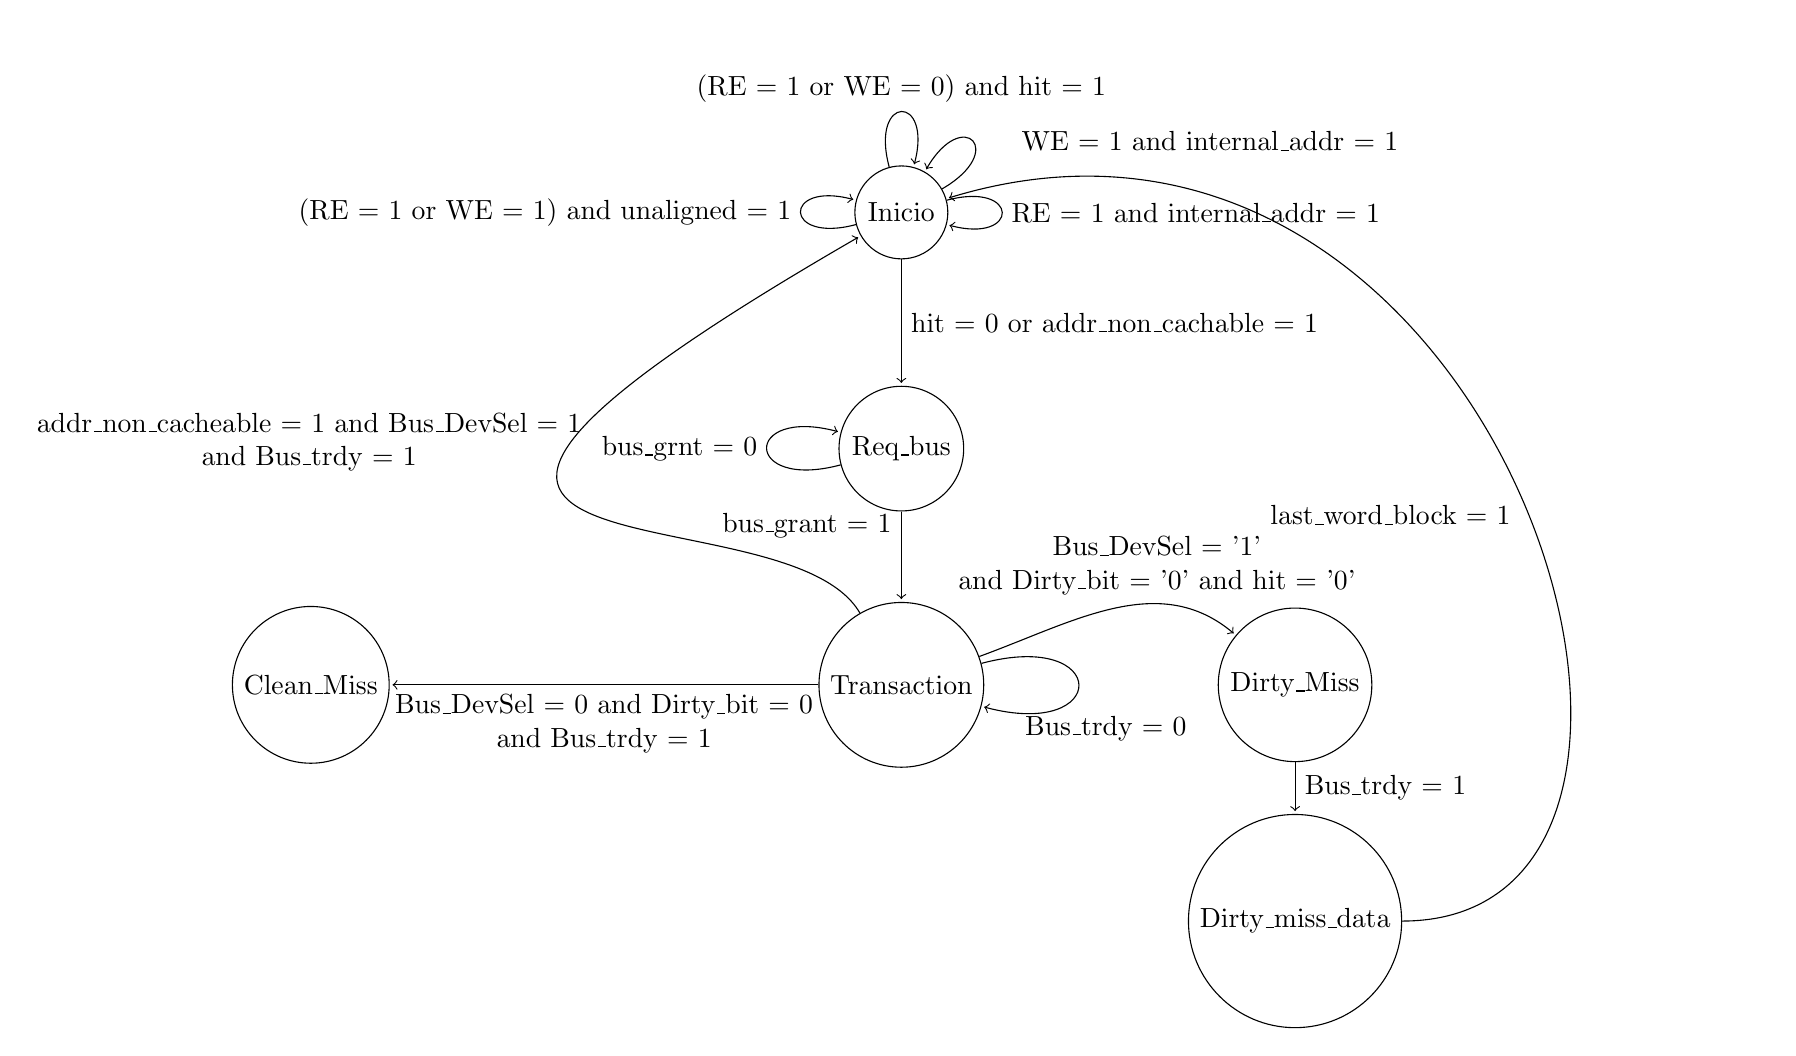
\begin{tikzpicture}[shorten >=1pt,node distance=3cm,on grid,auto,] 
   \node[state] (q_0)   {Inicio}; 
   \node[state] (q_1) [below=of q_0] {Req\_bus}; 
   \node[state] (q_2) [below=of q_1] {Transaction};
   \node[state] (q_4) [left=of q_2, xshift=-4.5cm] {Clean\_Miss};
   \node[state] (q_5) [left=of q_2, xshift=8cm] {Dirty\_Miss};
   \node[state] (q_6) [below=of q_5] {Dirty\_miss\_data};

    \path[->] 
    (q_0) edge  node {hit = 0 or addr\_non\_cachable = 1} (q_1)
          edge [loop above] node  {(RE = 1 or WE = 0) and hit = 1} ()
          edge [loop left]  node {(RE = 1 or WE = 1) and unaligned = 1} ()
          edge [loop right] node {RE = 1 and internal\_addr = 1} ()
          edge [out=30, in=60, looseness=8] node[right=0.5cm] {WE = 1 and internal\_addr = 1} (q_0)
    (q_1) edge  node[left, yshift=0.4cm]  {bus\_grant = 1} (q_2)
          edge [loop left] node {bus\_grnt = 0} ()
    (q_2) edge [loop right] node[xshift=-0.8cm, yshift=-0.55cm] {Bus\_trdy = 0} ()
          edge[out=160 , in=250, looseness=1, controls=+(120:3) and +(210:10)] node[align=center, yshift=1.4cm] {addr\_non\_cacheable = 1 and Bus\_DevSel = 1 \\ and Bus\_trdy = 1} (q_0)
          edge node[align=center] {Bus\_DevSel = 0 and Dirty\_bit = 0 \\ and Bus\_trdy = 1} (q_4)
          edge[out=20, in=140] node[align=center, pos=0.67] {Bus\_DevSel = '1' \\ and Dirty\_bit = '0' and hit = '0'} (q_5)
    (q_5) edge node {Bus\_trdy = 1} (q_6)
    (q_6) edge[out=270, in=15, looseness=3, controls=+(0:6) and +(17:8)] node {last\_word\_block = 1} (q_0);
\end{tikzpicture}
\end{adjustbox}
\end{center}

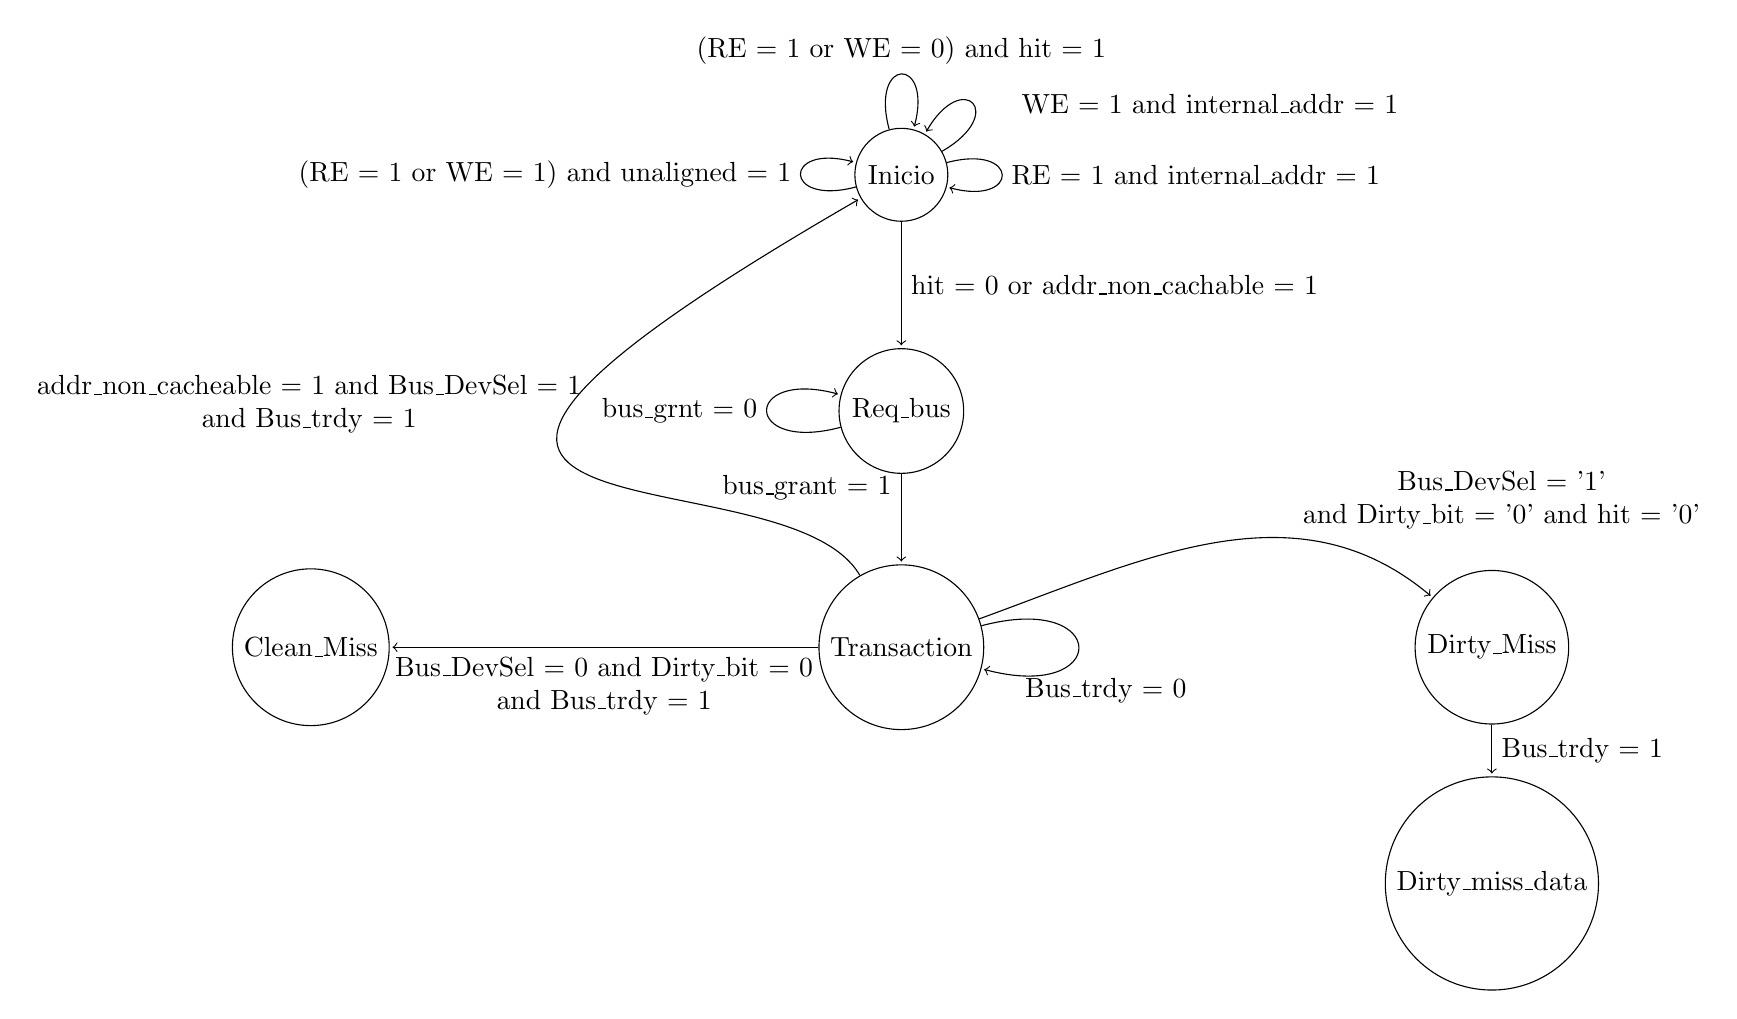
\begin{tikzpicture}[shorten >=1pt,node distance=3cm,on grid,auto] 
   \node[state] (q_0)   {Inicio}; 
   \node[state] (q_1) [below=of q_0] {Req\_bus}; 
   \node[state] (q_2) [below=of q_1] {Transaction};
   \node[state] (q_4) [left=of q_2, xshift=-4.5cm] {Clean\_Miss};
   \node[state] (q_5) [right=of q_2, xshift=4.5cm] {Dirty\_Miss};
   \node[state] (q_6) [below=of q_5] {Dirty\_miss\_data};

    \path[->] 
    (q_0) edge  node {hit = 0 or addr\_non\_cachable = 1} (q_1)
          edge [loop above] node  {(RE = 1 or WE = 0) and hit = 1} ()
          edge [loop left]  node {(RE = 1 or WE = 1) and unaligned = 1} ()
          edge [loop right] node {RE = 1 and internal\_addr = 1} ()
          edge [out=30, in=60, looseness=8] node[right=0.5cm] {WE = 1 and internal\_addr = 1} (q_0)
    (q_1) edge  node[left, yshift=0.4cm]  {bus\_grant = 1} (q_2)
          edge [loop left] node {bus\_grnt = 0} ()
    (q_2) edge [loop right] node[xshift=-0.8cm, yshift=-0.55cm] {Bus\_trdy = 0} ()
          edge[out=160 , in=250, looseness=1, controls=+(120:3) and +(210:10)] node[align=center, yshift=1.4cm] {addr\_non\_cacheable = 1 and Bus\_DevSel = 1 \\ and Bus\_trdy = 1} (q_0)
          edge node[align=center] {Bus\_DevSel = 0 and Dirty\_bit = 0 \\ and Bus\_trdy = 1} (q_4)
          edge[out=20, in=140] node[align=center, pos=0.67] {Bus\_DevSel = '1' \\ and Dirty\_bit = '0' and hit = '0'} (q_5)
    (q_5) edge node {Bus\_trdy = 1} (q_6);
\end{tikzpicture}




\newpage

\section{Descomposición de la Dirección de la cache}
Para direccionar nuestra memoria cache hemos optado por una descomposición en 8 bits, con los cuales podemos direccionar de la siguiente manera: 1 bit para direccionar entre los 2 sets (asociatividad 2), otro bit para direccionar entre las 2 vías que existen en cada set
, 2 bits que nos permiten direccionar bloques dentro de las vías, otros 2 bits para direccionar palabras dentro de estos bloques y por ultimo 2 bits para direccionar bytes dentro de la palabra. En nuestro caso como necesitamos direcciones alineadas estos 2 ultimos bits 
tendran siempre el mismo valor (00).\par
Diagrama descriptivo del direccionamiento de la cache:\par

\begin{figure}[htbp]
  \centering
  \includegraphics[page=1, width=0.8\textwidth, clip]{assets/Descomposicion_Direcciones_light.png}
  \caption{Descomposicion del direccionamiento de la MC}
  \label{fig:imagen}
\end{figure}

\section{Análisis de Latencias}
Para medir el rendimiento de la cache hemos utilizado una medición en ciclos, ya que es una medida de tiempo constante. Podríamos comparar la ejecucion del mismo programa 
en un procesador que no implementa cache y con uno que si lo hace. También podriamos medir los ciclos de reloj que espera la cpu a tener el dato listo. Factores a tener en cuenta 
sería el numero de fallos tanto en lectura como escritura ya que son estos los que hacen que nuestro procesador tenga que esperar al dato o instrucción, ralentizando la ejecución.\cite{HennyPatt}\par
Una manera sencilla de calcularlo sería\par

\begin{adjustwidth}{2cm}{2cm}
\vspace{15pt}
Tiempo de CPU = (Ciclos de reloj de ejecucion-CPU + Ciclos de reloj de detención memoria) · Duración de ciclo de reloj
\vspace{15pt}
\end{adjustwidth}

Para desgeneralizar el asunto podemos separar esta formula en varias para calcular partes individuales necesarias como serían los ciclos de detencion de memoria:

\begin{adjustwidth}{2cm}{2cm}
\vspace{15pt}
  Ciclos de reloj de detencion de memoria = $\frac{\text{Acceso a Memoria}}{\text{Programa}}$ · Frecuencia de fallos · Penalización de fallos
\vspace{15pt}
\end{adjustwidth}

Finalmente llegamos a la conclusión de que:

\begin{adjustwidth}{2cm}{2cm}
\vspace{15pt}
  Tiempo de CPU = IC · ( CPI$_{ejecucion}$ + $\frac{\text{Accesos a Memoria}}{\text{Instrucción}}$ · Frecuencia de fallos · Penalización de fallos) · Tiempo de ciclo de reloj
\vspace{15pt}
\end{adjustwidth}

\subsection{Ciclos Efectivos}
\lipsum[9-10]

\section{Programas de Prueba}
\lipsum[10-12]

\section{Ejemplo de Código}
\lipsum[13-14]

\section{Apartados Opcionales}
\subsection{Hacking Ético}
En este apartado hemos querido enseñar como podíamos realizar un ataque DOS (denial of service o denegación de servicio), si sabemos como esta estructurada la memoria cache de un procesador.\par
Para detectarlo, podríamos usar un contador de Write Missess, y que si ese valor es igual o muy cercano al numero de writes que se esta haciendo, saltar una señal alertando que posiblemente este tipo de ataque esta tendiendo lugar. 
Para solucionar esto lo que podríamos hacer es implementar un bit de lock, de manera que ciertas instrucciones que podamos marcar, no abandonarían nunca la cache. Mejorando el rendimiento del procesador frente a este tipo de ataques. Otra solución podría ser mandar un 
halt de manera que terminaríamos este proceso (en caso de que la procesador sea uniciclo). 
Información sobre este tipo de ataque: \cite{BackCache}.

\section{Horas Dedicadas}

\begin{table}[h]
\centering
\begin{tabularx}{\textwidth}{|X|}
\hline
\horasDepuracion{0}{0} \\
\hline
\horasEntenderEnunciado{2}{1} \\
\hline
\horasMemoria{2}{0} \\
\hline
\horasVhdl{7}{3} \\
\hline
\end{tabularx}
\end{table}

\section{Autoevaluación}
\lipsum[15-18]

\newpage
\section{Anexo}
\subsection{Imágenes}
\begin{figure}[htbp]
  \centering
  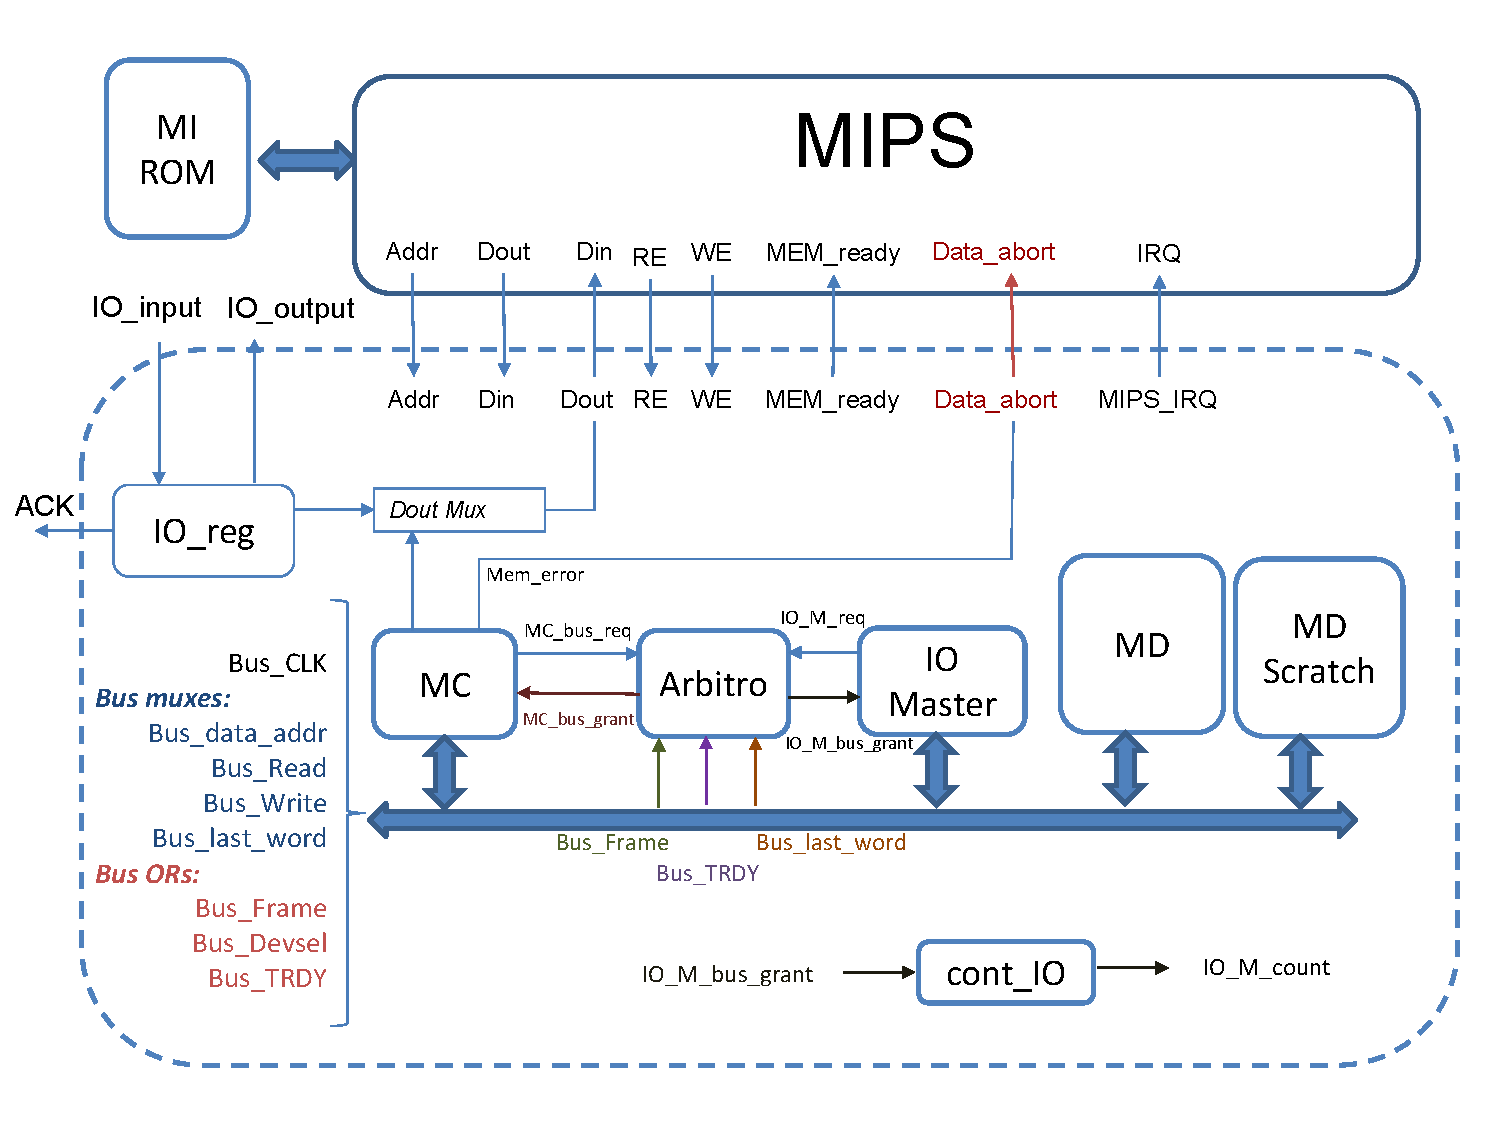
\includegraphics[page=1, width=0.8\textwidth, clip]{assets/AOC2_2024_Esquemas_Proy2.pdf}
  \caption{Esquema y señales principales del nuevo IO MD subsytem y de su bus. Se pide diseñar la
Unidad de Control de la MC}
  \label{fig:imagen}
\end{figure}

\newpage
\bibliographystyle{apalike}
\bibliography{assets/biblio} % Enlaza al archivo de bibliografía sin la extensión .bib



\end{document}

